% Standalone HBF: 28 Oct 2026 Research Meeting
% Visual style follows the 21 Oct 2026 light Madrid decks.
% Quantitative evidence is limited to the task brief and verified figure content.
% Compile with pdfLaTeX from this directory. Keep CharacterizationOfHBFforKVCentricLLMServing/ beside this file.
\documentclass[aspectratio=169,10pt]{beamer}
\usepackage[english]{babel}
\usepackage[utf8]{inputenc}
\usepackage[T1]{fontenc}
\usepackage{lmodern}
\usepackage{amsmath,amssymb}
\usepackage{booktabs,tabularx,array}
\usepackage{graphicx}
\graphicspath{{./}{figures/}}
\usepackage{xcolor}
\usepackage{tikz}
\usetikzlibrary{arrows.meta,positioning,calc,shapes.geometric}
\usepackage{hyperref}

\usetheme{Madrid}
\usecolortheme{default}
\definecolor{Ink}{HTML}{243748}
\definecolor{Muted}{HTML}{667B8B}
\definecolor{Accent}{HTML}{347E74}
\definecolor{AccentBlue}{HTML}{507DAD}
\definecolor{SoftMint}{HTML}{E6F4EE}
\definecolor{SoftBlue}{HTML}{E9F2F9}
\definecolor{SoftLilac}{HTML}{F1EEF8}
\definecolor{Paper}{HTML}{FBFCFE}
\definecolor{Divider}{HTML}{D8E4EB}

\setbeamercolor{background canvas}{bg=Paper}
\setbeamercolor{normal text}{fg=Ink}
\setbeamercolor{structure}{fg=Accent}
\setbeamercolor{frametitle}{fg=Ink,bg=SoftBlue}
\setbeamercolor{title}{fg=Ink}
\setbeamercolor{subtitle}{fg=Muted}
\setbeamercolor{block title}{fg=Ink,bg=SoftBlue}
\setbeamercolor{block body}{fg=Ink,bg=white}
\setbeamercolor{item}{fg=Accent}
\setbeamercolor{caption name}{fg=Muted}
\setbeamercolor{footline}{fg=Muted,bg=Paper}
\setbeamerfont{frametitle}{size=\large,series=\bfseries}
\setbeamerfont{footline}{size=\tiny}
\setbeamerfont{block title}{series=\bfseries}
\setbeamertemplate{headline}{}
\setbeamertemplate{navigation symbols}{}
\setbeamertemplate{blocks}[rounded][shadow=false]
\setbeamertemplate{itemize items}[circle]
\setbeamertemplate{itemize subitem}[circle]
\setbeamertemplate{footline}{%
  \leavevmode\hbox{%
    \begin{beamercolorbox}[wd=\paperwidth,ht=.30cm,dp=.16cm,rightskip=.60cm plus 1fil]{footline}%
      \hfill\insertframenumber\,/\,\inserttotalframenumber
    \end{beamercolorbox}}}
\setbeamertemplate{frametitle}{%
  \nointerlineskip
  \begin{beamercolorbox}[wd=\paperwidth,ht=.72cm,dp=.16cm,leftskip=.55cm,rightskip=.40cm]{frametitle}%
    \usebeamerfont{frametitle}\insertframetitle
  \end{beamercolorbox}}

\newcommand{\smalllabel}[1]{{\scriptsize\bfseries\color{Accent}\MakeUppercase{#1}}}
\newcommand{\hint}[1]{{\scriptsize\color{Muted}#1}}
\newcommand{\takeaway}[1]{%
  \begin{beamercolorbox}[rounded=true,sep=0.12cm,wd=\linewidth]{block title}%
    {\small\bfseries #1}
  \end{beamercolorbox}}
\newcommand{\stepcard}[3]{%
  \begin{beamercolorbox}[rounded=true,sep=0.10cm,wd=\linewidth]{block body}%
    {\scriptsize\bfseries\color{Accent}#1}\par\vspace{.4mm}
    {\footnotesize\bfseries #2}\par\vspace{.4mm}
    {\scriptsize\color{Muted}#3}%
  \end{beamercolorbox}}

\newcommand{\figureplaceholder}[3]{%
  \begingroup\centering
  \IfFileExists{#1}{%
    \includegraphics[width=.98\linewidth,height=#2,keepaspectratio]{#1}%
  }{%
    \IfFileExists{figures/#1}{%
      \includegraphics[width=.98\linewidth,height=#2,keepaspectratio]{figures/#1}%
    }{%
      \begin{tikzpicture}
        \node[draw=AccentBlue!55,dashed,line width=.7pt,rounded corners=4pt,
              fill=SoftBlue!60,minimum height=#2,minimum width=.95\linewidth,
              text width=.85\linewidth,align=center,inner sep=2mm] {
           {\color{AccentBlue}\bfseries FIGURE PLACEHOLDER}\\[2.2mm]
           {\color{Ink}\small #3}\\[1.5mm]
           {\color{Muted}\scriptsize\ttfamily\detokenize{#1}}};
      \end{tikzpicture}%
    }%
  }\par\endgroup}

\newcommand{\src}[1]{\vspace{0.05cm}\hint{Source: #1}}

\title[HBF]{HBF Sucks?}
\author{Yu-Jui Liang}
\date{28 Oct 2026}
\subject{Research meeting, 28 Oct 2026}
\begin{document}
{\setbeamertemplate{footline}{}
\begin{frame}[plain]
\vspace*{.45cm}
\smalllabel{Research meeting / paper summary}\par\vspace{.3cm}
{\LARGE\bfseries HBF Sucks?\par}\vspace{.14cm}
{\Large\bfseries A Full-Stack Characterization of High-Bandwidth Flash\\[.1cm]
for KV-Centric LLM Serving\par}\vspace{.35cm}
{\large\color{Accent}A faster flash tier can make the serving system slower.\par}
\vspace{.55cm}
{\bfseries Yu-Jui Liang}\par
{\small\color{Muted}Advisor: Hsiang-Yun Cheng}\par
{\small\color{Muted}National Taiwan University \quad | \quad Academia Sinica \quad | \quad 28 Oct 2026}\par
\vfill
{\scriptsize\color{Muted}Zhuoran Li, Zhuohang Bian, Xin Huang, Yibo Zhao, Guangyu Sun, Youwei Zhuo\par
arXiv:2608.11668v4}\par\vspace{.08cm}
{\color{Accent}\rule{\textwidth}{.7pt}}
\end{frame}}

\begin{frame}[t]{Why Replace SSD with HBF?}
\smalllabel{Motivation / the intuitive upgrade}\par\vspace{.18cm}
\begin{columns}[T,onlytextwidth]
\begin{column}{.57\textwidth}
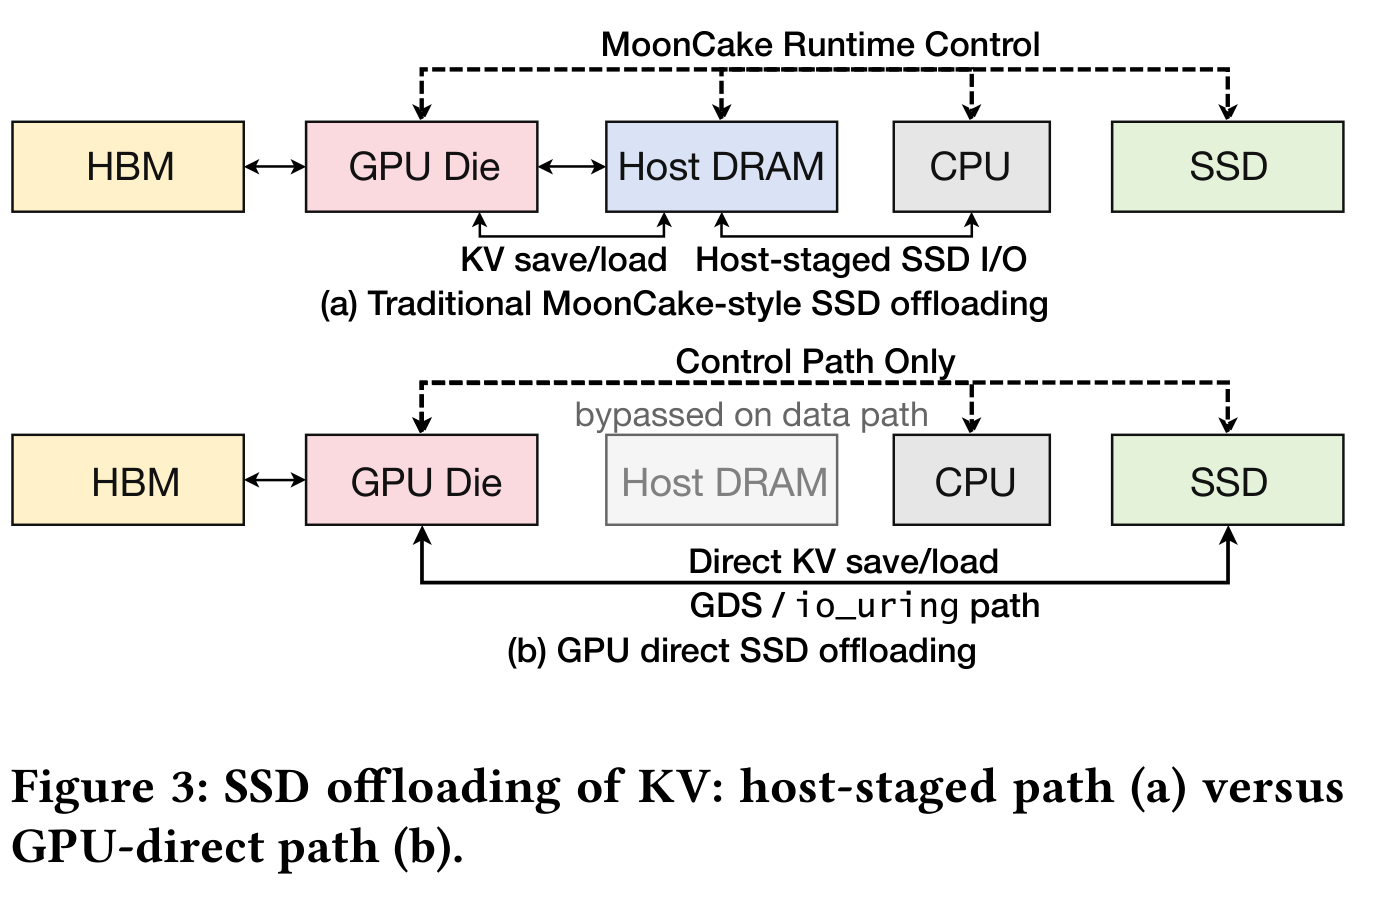
\includegraphics[width=\linewidth,height=4.25cm,keepaspectratio]{CharacterizationOfHBFforKVCentricLLMServing/Figure_03_SSD_KV_offloading_paths.png}
\end{column}
\begin{column}{.40\textwidth}
\textbf{KV cache outgrows GPU memory}\par
\small Save / load KV to an SSD backing tier, through host staging or GPU-direct I/O.\par\vspace{.22cm}
\textbf{HBF promises faster flash}\par
Package-local flash offers lower latency and higher bandwidth.\par\vspace{.3cm}
{\normalsize\bfseries Does faster flash translate into faster end-to-end LLM serving?\par}
\end{column}
\end{columns}
\vfill\takeaway{The paper tests the intuitive ``SSD $\rightarrow$ HBF'' upgrade at the full-system level.}
\src{Fig. 3, abstract and introduction.}
\end{frame}

\begin{frame}[t]{What Did the Paper Actually Evaluate?}
\smalllabel{Method / drop-in substitution}\par\vspace{.18cm}
\begin{columns}[T,onlytextwidth]
\begin{column}{.49\textwidth}
\textbf{Keep the Mooncake-style runtime}\par
\small Admission / retention / lookup / KV save \& restore\par\vspace{.12cm}
\textbf{Swap capacity-matched SSD for HBF-1 / HBF-2}
\end{column}
\begin{column}{.48\textwidth}
\textbf{Extended TokenSim}\par
\small 4 complete two-hour traces; 5 dense / MoE models\\
H100 / B200 profiles; thermal + endurance models
\end{column}
\end{columns}

\vspace{.20cm}
\begin{columns}[T,onlytextwidth]
\begin{column}{.60\textwidth}
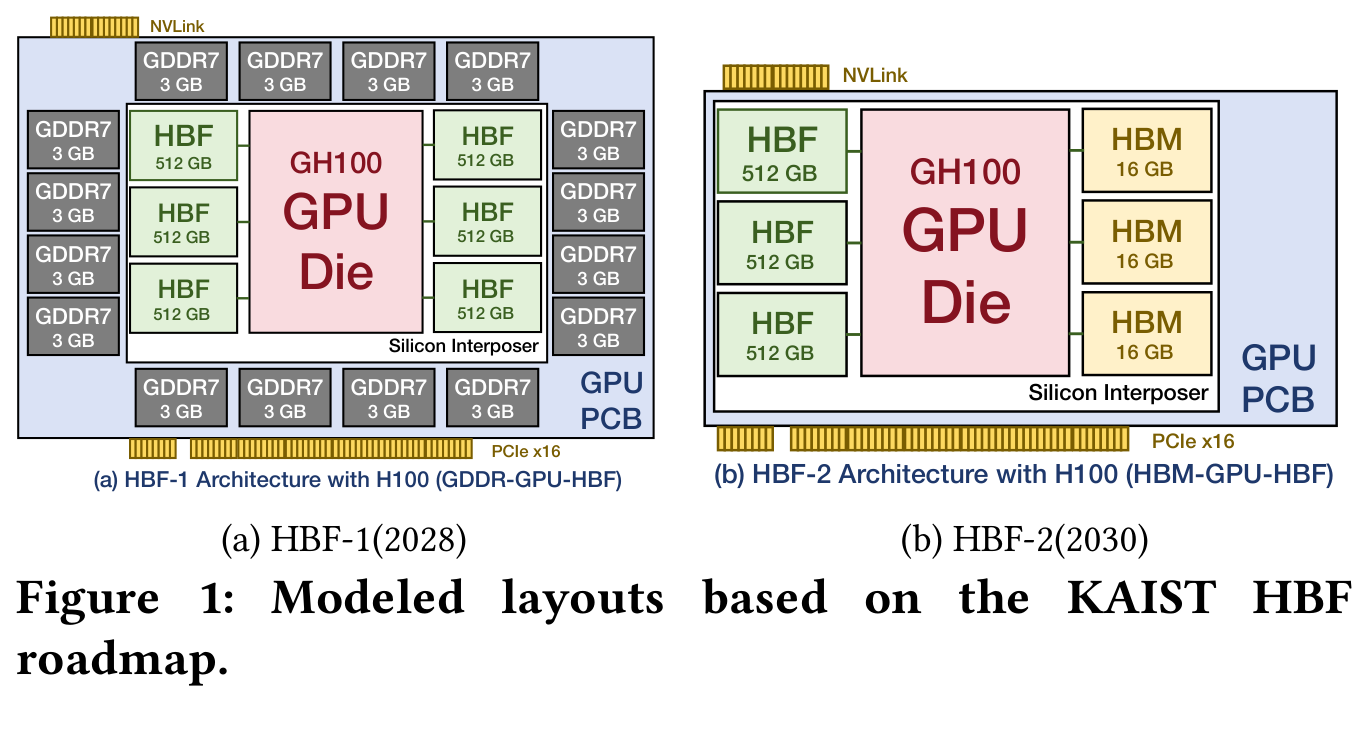
\includegraphics[width=\linewidth,height=3.5cm,keepaspectratio]{CharacterizationOfHBFforKVCentricLLMServing/Figure_01_HBF1_HBF2_roadmap_layouts.png}
\end{column}
\begin{column}{.37\textwidth}
\small\textbf{HBF-1 (2028): GDDR--GPU--HBF}\par
Interposer sites go to HBF; near tier moves to off-interposer GDDR7.\par\vspace{.15cm}
\textbf{HBF-2 (2030): HBM--GPU--HBF}\par
HBM and HBF share sites; near-tier HBM capacity / bandwidth falls vs. SSD baseline.
\end{column}
\end{columns}
\vfill\takeaway{HBF trades near-tier resources for package-local flash.}
\src{Fig. 1, Tables 2 and 3(c), Sec. 6.1. Roadmap profiles + TokenSim + 3D-ICE + endurance model.}
\end{frame}

\begin{frame}[t]{Three Conditions for HBF to Help}
\smalllabel{Organizing principle}\par\vspace{.55cm}
\begin{columns}[T,onlytextwidth]
\begin{column}{.31\textwidth}
\begin{block}{C1 --- Critical Path}
\normalsize Read I/O must be a real serving bottleneck.\par\vspace{.25cm}
\hint{F1--F2: package tradeoff and limited base-die compute leverage.}
\end{block}
\end{column}
\begin{column}{.31\textwidth}
\begin{block}{C2 --- Reuse}
\normalsize Useful reads must repay every HBF write.\par\vspace{.25cm}
\hint{F3--F4: cold write-heavy traffic and limited batching benefit.}
\end{block}
\end{column}
\begin{column}{.31\textwidth}
\begin{block}{C3 --- Sustainability}
\normalsize High bandwidth must remain sustainable.\par\vspace{.25cm}
\hint{F5--F6: thermal throttling and flash write wear.}
\end{block}
\end{column}
\end{columns}
\vspace{.45cm}
\centering\textbf{6 findings = 2 findings for each condition}\par
\vfill\takeaway{A faster medium helps only if all three conditions hold.}
\src{Sections 5--8.}
\end{frame}

\begin{frame}[t]{Faster HBF Barely Improves E2E Latency}
\smalllabel{C1 fails / flash is barely on the critical path}\par\vspace{.10cm}
{\centering
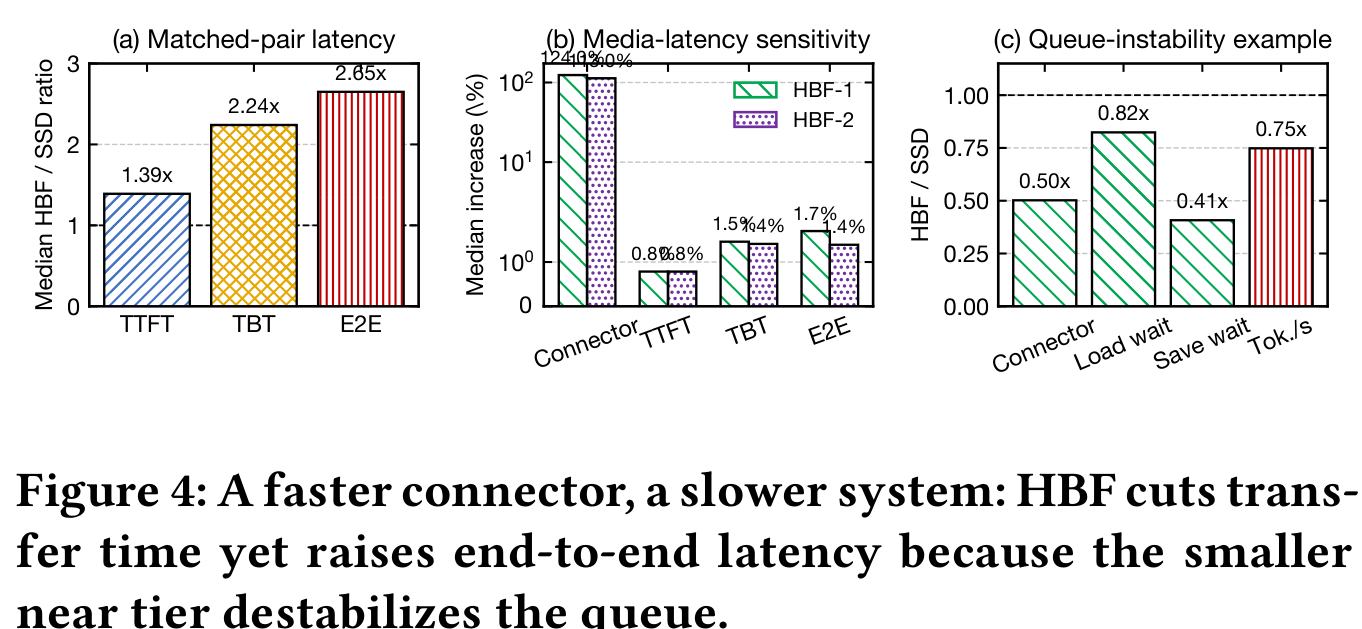
\includegraphics[width=.90\linewidth,height=3.7cm,keepaspectratio]{CharacterizationOfHBFforKVCentricLLMServing/Figure_04_faster_connector_slower_system.png}
\par}\vspace{.12cm}
\begin{columns}[T,onlytextwidth]
\begin{column}{.48\textwidth}
\small Mean E2E latency = \textbf{2--5.5$\times$ SSD baseline}\par
Less near-tier capacity / bandwidth\par
$\rightarrow$ fewer admitted requests, more queueing
\end{column}
\begin{column}{.49\textwidth}
\small \textbf{3.75$\times$ faster raw HBF latency}\par
$\rightarrow$ E2E only \textbf{0.75\% / 0.88\%} lower (HBF-1 / 2)\par
$\rightarrow$ exposed secondary-tier I/O $\approx$ \textbf{1\%}
\end{column}
\end{columns}
\vfill\takeaway{The bottleneck is not flash-media latency.}
\src{Fig. 4 and Sec. 6.1. HBF-1 vs. SSD24; HBF-2 vs. SSD12. H100/B200 simulation.}
\end{frame}

\begin{frame}[t]{All Production Traces Send More Writes Than Reads to HBF}
\smalllabel{C2 fails / useful reads do not repay writes}\par\vspace{.3cm}
{\normalsize\renewcommand{\arraystretch}{1.45}
\begin{tabularx}{\linewidth}{@{}l*{4}{>{\centering\arraybackslash}X}@{}}
\toprule
\textbf{Metric} & \textbf{traceA} & \textbf{traceB} & \textbf{coder} & \textbf{thinking}\\
\midrule
Write/read ratio & $2.14\times$ & $4.90\times$ & $1.14\times$ & $2.20\times$\\
$\rho$ = reads/write & 0.47 & 0.20 & 0.88 & 0.45\\
Prefix hit rate & 38.21\% & 52.46\% & 45.58\% & 44.12\%\\
\bottomrule
\end{tabularx}}\par\vspace{.1cm}
\hint{Table 8: flash-tier byte traffic over each full two-hour replay.}\par\vspace{.3cm}
\begin{columns}[T,onlytextwidth]
\begin{column}{.52\textwidth}
\small Hot, highly reused KV $\rightarrow$ retained in HBM / GDDR\par\vspace{.12cm}
Cold, low-reuse KV $\rightarrow$ evicted to HBF
\end{column}
\begin{column}{.44\textwidth}
\small Prefix reuse exists, but stays in the near tier.\par\vspace{.12cm}
Every trace writes more bytes than it reads from HBF.
\end{column}
\end{columns}
\vfill\takeaway{The cache hierarchy gives HBF a write-heavy, low-reuse KV stream.}
\src{Table 8 and Sec. 7.1. Production-trace replay, not HBF device measurements.}
\end{frame}

\begin{frame}[t]{Write-Heavy KV Traffic Makes Peak HBF Bandwidth Unsustainable}
\smalllabel{C3 fails / thermal limits and write wear}\par\vspace{.08cm}
\begin{columns}[T,onlytextwidth]
\begin{column}{.55\textwidth}
\raggedright
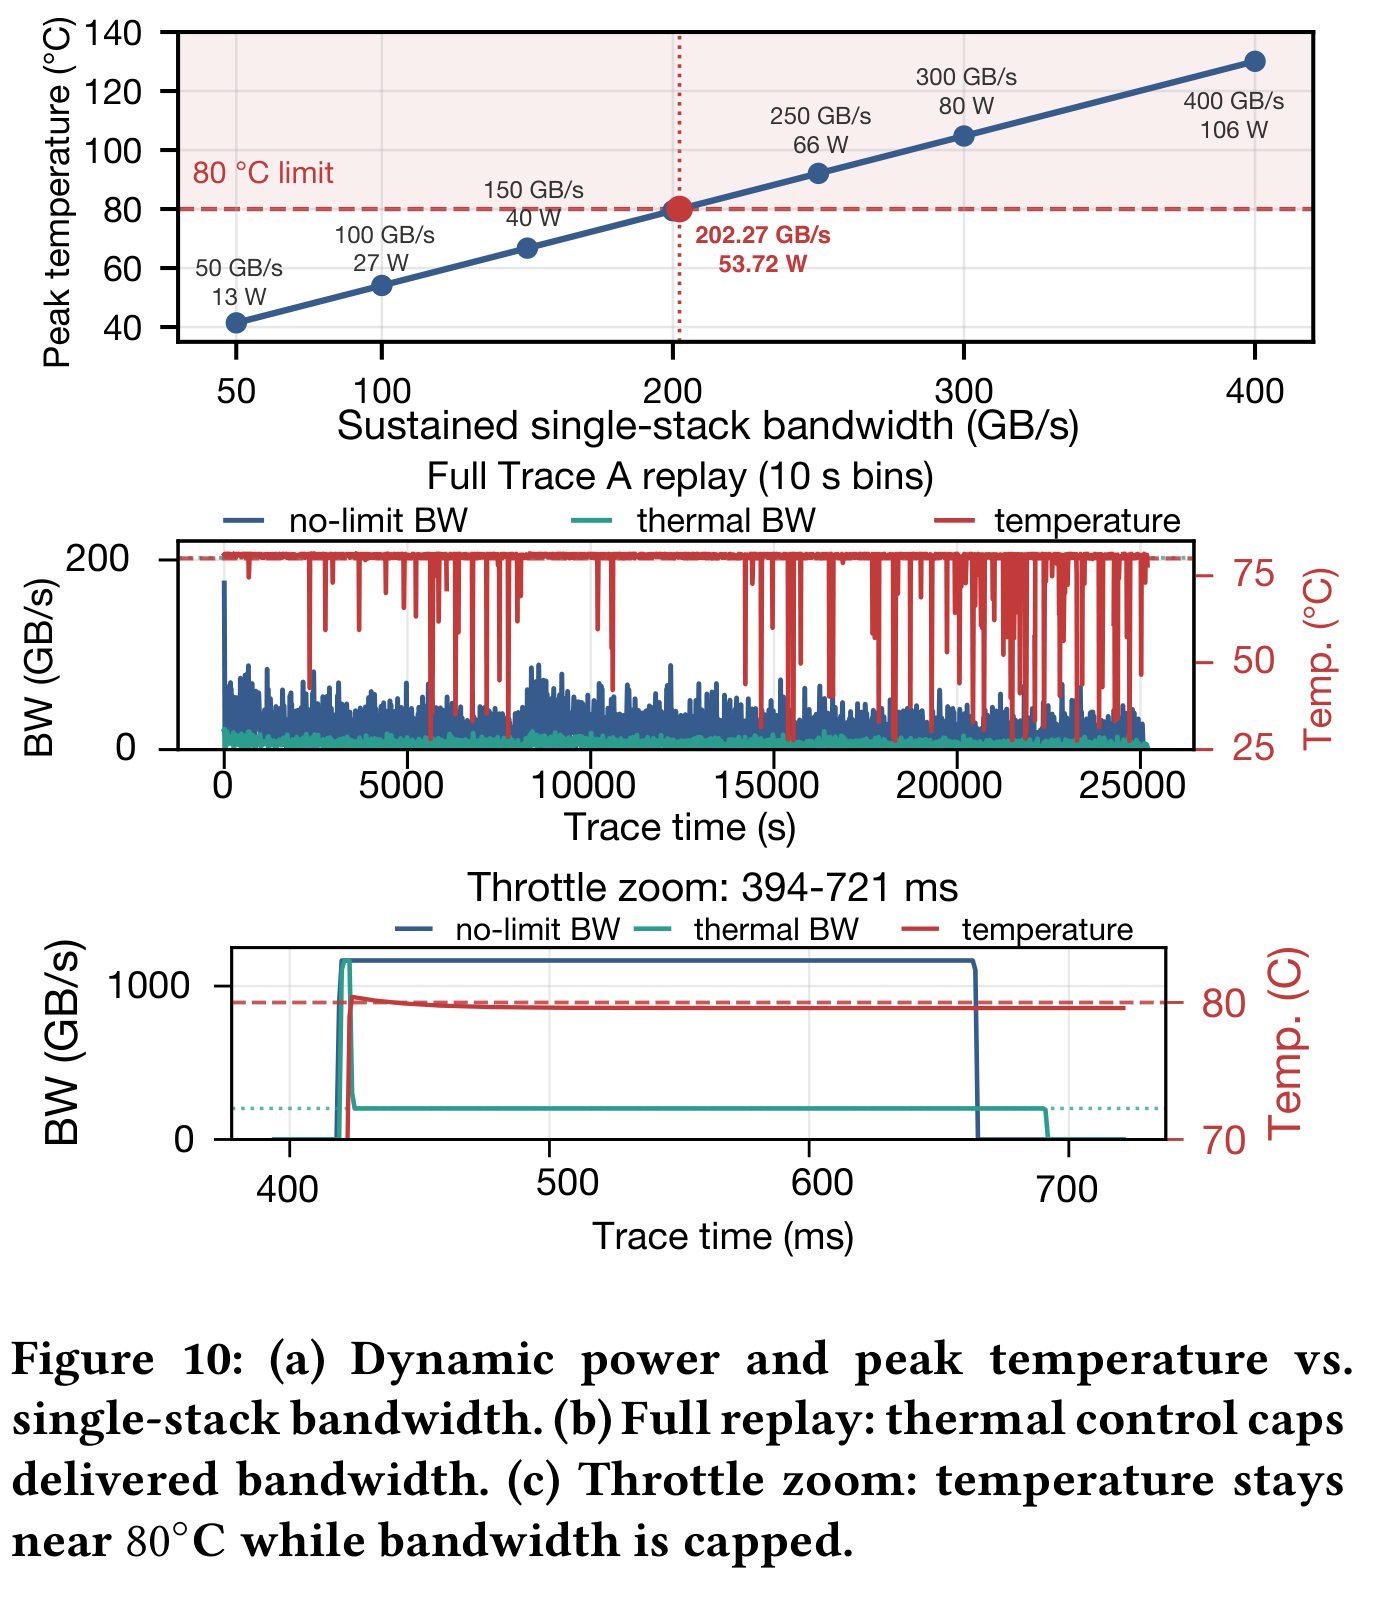
\includegraphics[width=\linewidth,height=5.0cm,keepaspectratio]{CharacterizationOfHBFforKVCentricLLMServing/Figure_10_HBF_thermal_throttling.png}
\end{column}
\begin{column}{.42\textwidth}
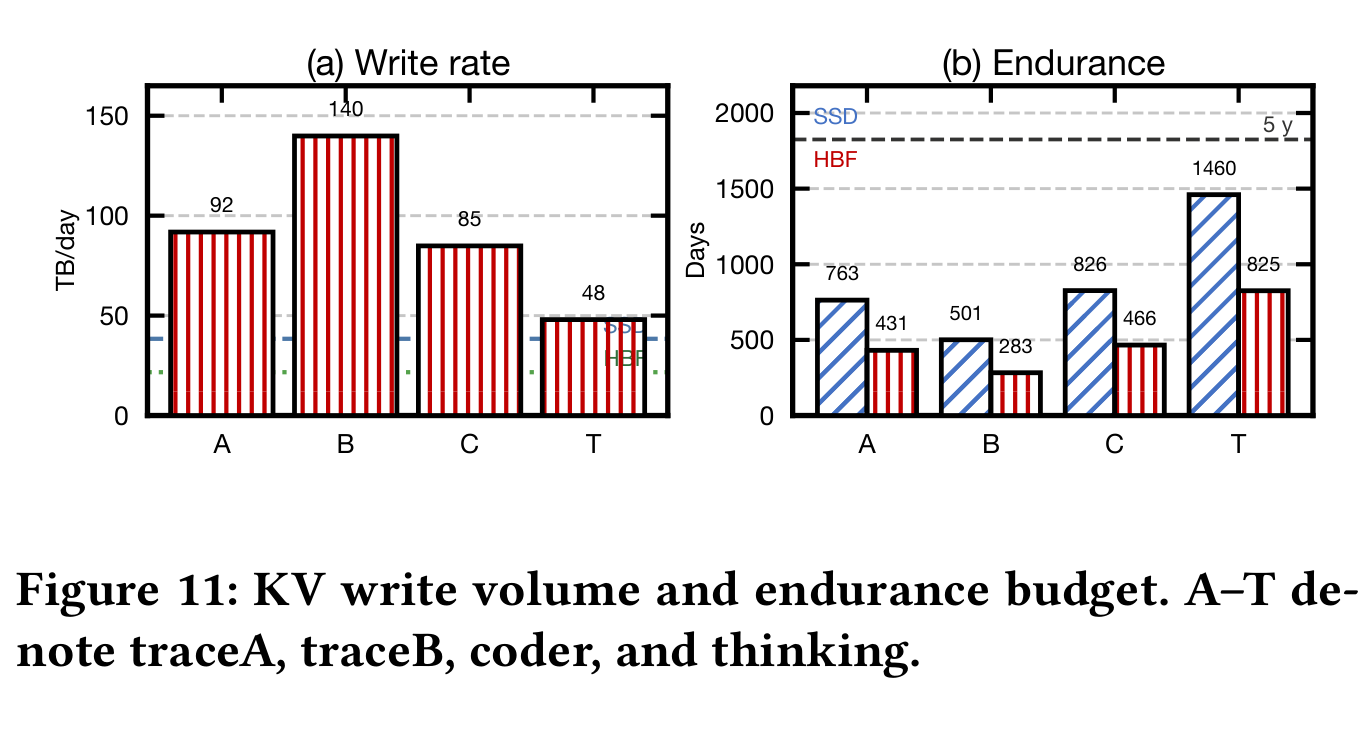
\includegraphics[width=\linewidth,height=2.25cm,keepaspectratio]{CharacterizationOfHBFforKVCentricLLMServing/Figure_11_KV_write_endurance.png}\par\vspace{.12cm}
\small\textbf{Short term: thermal throttling}\par
\textbf{202.27 GB/s} at \textbf{80$^\circ$C}\par Delivered BW $<$ peak (16-Hi TLC).\par\vspace{.18cm}
\textbf{Long term: write endurance}\par
Trace writes: \textbf{48--140 TB/day}\par
Modeled HBF lifetime $\approx$ \textbf{0.56$\times$ SSD}\par

\end{column}
\end{columns}
\vfill\takeaway{Write-heavy KV reduces sustained bandwidth and consumes flash lifetime.}
\src{Figs. 10--11 and Sec. 8. Model projections, not hardware lifetime measurements.}
\end{frame}

\begin{frame}[t]{The Device Is Fine; the Drop-In Deployment Is Not}
\smalllabel{Conclusion / placement requirements}\par\vspace{.15cm}
\begin{columns}[T,onlytextwidth]
\begin{column}{.55\textwidth}
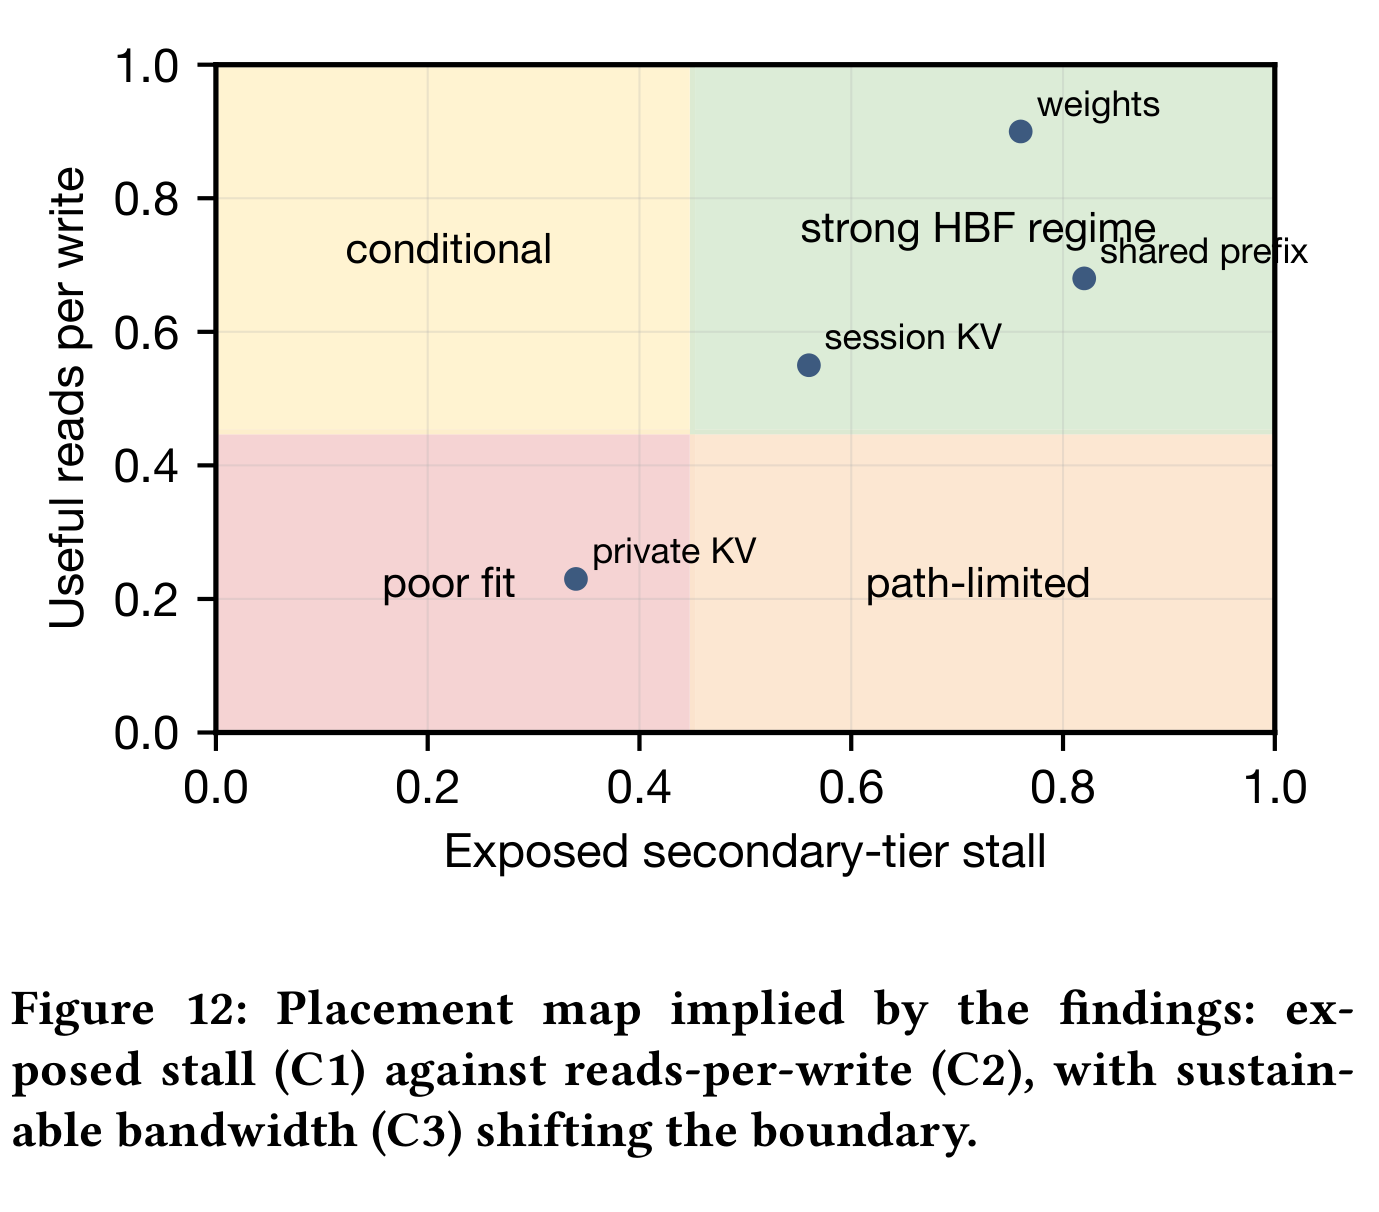
\includegraphics[width=\linewidth,height=4.3cm,keepaspectratio]{CharacterizationOfHBFforKVCentricLLMServing/Figure_12_HBF_placement_map.png}

\end{column}
\begin{column}{.42\textwidth}
\begin{columns}[T,onlytextwidth]
\begin{column}{.49\textwidth}
\small\textbf{Poor HBF targets}\par\small
Private KV\\Transient decode KV\\Low-reuse objects
\end{column}
\begin{column}{.49\textwidth}
\small\textbf{Better HBF targets}\par\small
Model weights\\Shared prefixes\\Read-mostly objects
\end{column}
\end{columns}
\vspace{.2cm}
\textbf{Requirements for a future runtime}\par\vspace{.1cm}
\small Critical-path-aware / reuse-aware\\Write-budgeted / thermal-aware
\end{column}
\end{columns}
\vspace{.15cm}
\takeaway{HBF should not be treated as a faster SSD.}
\vspace{.1cm}\small A conceptual design map from the findings, not an implemented runtime or calibrated boundary.\par
\src{Fig. 12 and Sections 9--10.}
\end{frame}

% ----- SLIDE 09: Sources after the main conclusion -----
\begin{frame}[t]{Sources Behind the HBF Evaluation}
\vspace{0cm}
\begin{columns}[T,onlytextwidth]
\begin{column}{.30\textwidth}
\smalllabel{System / workload}\par\vspace{.06cm}
\textbf{\href{https://github.com/pku-lemonade/TokenSim}{TokenSim} / \href{https://github.com/pku-lemonade/TokenSim/tree/hbf}{HBF code}}\par
\footnotesize pku-lemonade research project\\
Open-source serving simulator\par
$\rightarrow$ Serving, KV transfers, queueing and E2E latency\par\vspace{.27cm}
\normalsize\textbf{\href{https://www.usenix.org/conference/atc25/presentation/wang-jiahao}{Qwen-Bailian traces}}\par
\footnotesize Alibaba / SJTU; production data\par
$\rightarrow$ Request and reuse replay:\\
traceA, traceB, coder, thinking
\end{column}
\begin{column}{.37\textwidth}
\smalllabel{HBF definition}\par\vspace{.06cm}
\textbf{\href{https://www.opencompute.org/contributions/?project=Storage}{OCP HBF v0.7.0}}\par
\footnotesize Open Compute Project --- \textbf{industry spec}\\
Contributors: Sandisk + SK hynix\par
$\rightarrow$ Interface, page-write and lifecycle rules\par\vspace{.06cm}
\normalsize\textbf{\href{https://tera.kaist.ac.kr/}{KAIST HBF roadmap}}\par
\footnotesize Joungho Kim / KAIST TERA Lab\par
$\rightarrow$ HBF-1 / HBF-2 organizations\par
\textbf{Academic roadmap, not a product datasheet}\par\vspace{.06cm}
\normalsize\textbf{\href{https://arxiv.org/abs/2603.01175}{HAVEN}}\par
\footnotesize Hsu et al.; academic architecture/model\par
$\rightarrow$ NAND latency, energy, bandwidth, power
\end{column}
\begin{column}{.29\textwidth}
\smalllabel{Physical limits}\par\vspace{.06cm}
\textbf{\href{https://github.com/esl-epfl/3d-ice}{3D-ICE}}\par
\footnotesize EPFL; open-source thermal tool\par
$\rightarrow$ 16-Hi HBF temperature model\par
\hint{80$^\circ$C policy: chosen by this paper.}\par\vspace{.27cm}
\normalsize\textbf{\href{https://americas.kioxia.com/content/dam/kioxia/en-us/business/ssd/oem/supermicro/asset/KIOXIA_Supermicro_SSD_Data_Sheet_Global.pdf}{KIOXIA CM7-V data}}\par
\footnotesize KIOXIA America; vendor datasheet\par
$\rightarrow$ SSD baseline / rated endurance\par
\hint{HBF lifetime: authors' TLC budget + trace writes; not a wear-out test.}
\end{column}
\end{columns}
\vspace{.06cm}
\hint{2028 / 2030 are roadmap generations, not guaranteed mass-production dates.}\par
\vfill\takeaway{No physical HBF hardware is measured here: the full-stack model combines code, specifications, roadmaps, device models, production traces and thermal modeling.}
\src{Paper Refs. [1], [9], [11], [13], [23], [24], [26]; Sections 2 and 4.}
\end{frame}
\end{document}
